\section{Compilation}
\label{sec:compilation}

\begin{figure}
	\centering

	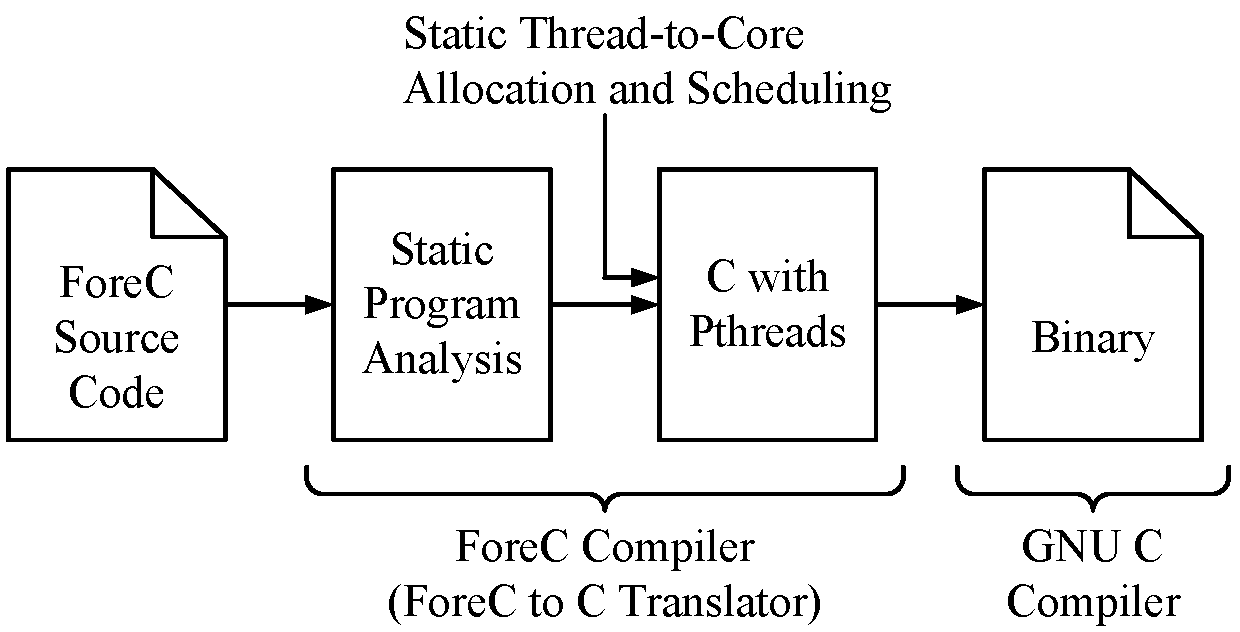
\includegraphics[width=0.6\columnwidth]{images/compilation_overview.pdf}

	\caption{Overview of compiling ForeC programs.}
	\label{fig:compilation_overview}
\end{figure}

Our ForeC compiler 
generates code for direct (bare metal) execution on embedded
multicores. Figure~\ref{fig:compilation_overview} is
an overview of the compilation process. The first step is to
check the syntax of the ForeC source code. This includes
checking whether all threads have been defined and whether
all variables accessed by multiple threads have been
declared with the \verb$shared$ qualifier. The second step
is to translate the ForeC statements into equivalent C code.
Startup and thread scheduling routines are generated for
each core. The ForeC threads are statically allocated and
statically scheduled on each core.
The advantages with our static scheduling approach include: 
(1) light-weight thread scheduling, and 
(2) easier debugging because all scheduling decisions are known beforehand.
However, the disadvantages include:
(1) needing to recompile to target different numbers of cores, and
(2) inability to dynamically load balance the ForeC threads to utilize idle cores.
The final step is to compile the generated 
C program with a GNU C compiler because GNU-specific 
computed \verb$goto$s are used to implement
thread context-switching. In comparison, compilers for
traditional synchronous languages typically compile away
concurrency to generate only sequential code~\cite{timed_cec}.
This is because concurrency in traditional synchronous 
languages is a logical concept, rather than a specification
for parallel execution. The rest of this section describes
the translation of ForeC to C code. 
For brevity, we omit inputs and outputs 
because we follow existing approaches~\cite{timed_compiling_esterel} for
creating the reactive interface.

\subsection{Structure of the Generated Program}
Figure~\ref{fig:compilation_example3_forec} is a small ForeC
program and Figure~\ref{fig:compilation_example3_c1} is a
simplified version of the generated C program. Hereafter, all line
numbers refer explicitly to
Figure~\ref{fig:compilation_example3_c1}.
The generated
C program contains global declarations and functions from the ForeC program
(lines~\ref{code:compilation_example3_user1}-\ref{code:compilation_example3_user2}), 
global declarations for implementing the
scheduling and shared variables 
(lines~\ref{code:compilation_example3_scheduling1}-\ref{code:compilation_example3_copies}
and \ref{code:compilation_example3_scheduling3}-\ref{code:compilation_example3_scheduling4}), 
a \verb$main$ function function (line~\ref{code:compilation_example3_forecmain})
containing all the static scheduling routines 
(lines~\ref{code:compilation_example3_scheduler1}-\ref{code:compilation_example3_scheduler2}) 
and ForeC threads (lines~\ref{code:compilation_example3_threads1}-\ref{code:compilation_example3_threads2}). 
When each core executes, it is directed to its own scheduling routine 
(lines~\ref{code:compilation_example3_direct1}-\ref{code:compilation_example3_direct2}),
which controls when its allocated ForeC threads are
executed. The threads and scheduling routines are inlined
into the \verb$main$ function because fast context-switching can be
implemented by jumping between C labels. All variables in
the threads are given unique names and hoisted up to
the \verb$main$ function's top scope (e.g., \verb$tC$'s local variable
\verb$a$ on line~\ref{code:compilation_example3_a}). 
This avoids the need to create
stacks for each thread to maintain their local variables.
However, all functions on the same core will
share the same stack space. To avoid stack corruption, all
functions must execute atomically, i.e., cannot be preempted
by other threads. In
future versions of the compiler, we wish to remove this
limitation by creating proper thread stacks.

\begin{figure}
	\centering

	\begin{minipage}{0.47\columnwidth}
		\subfloat[Example ForeC program.]{
			\lstinputlisting[style=full]{./code/example3.forec}
			\label{fig:compilation_example3_forec}	
		}
	\end{minipage}
	\hspace{1cm}
	\begin{minipage}{0.2\columnwidth}
		\centering
		\subfloat[Total order.]{
			
\includegraphics[width=0.7\columnwidth]{images/total_order.pdf}
			\label{fig:compilation_total_order}	
		}
		\vspace{1cm}
		\subfloat[Thread allocation.]{
			\renewcommand{\arraystretch}{1.25}
			\begin{tabular}{| l | l |}
				\hline
				{\bf Core 1}	& {\bf Core 2}	\\
				\hline
				main			& tD			\\
				tA				& tB			\\
				tC				&				\\
				\hline
			\end{tabular}
			\label{fig:compilation_schedule}	
		}
	\end{minipage}
	\caption{Example of compiling a ForeC program.}
\end{figure}

\begin{figure}
	\centering

	\lstinputlisting[style=fulltight,multicols=2,frame=tlr,lastline=138]{./code/example3.c}

	\caption{Example C program (continued).}
	\label{fig:compilation_example3_c1}
\end{figure}

\begin{figure}
	\ContinuedFloat 
	\centering

	\lstinputlisting[style=fulltight,multicols=2,frame=lrb,firstline=139,firstnumber=139]{./code/example3.c}

	\caption{Example C program.}
	\label{fig:compilation_example3_c2}
\end{figure}

\subsection{Static Thread Scheduling}
The rest of this section is exclusively about
ForeC threads. Hereafter, for brevity, ForeC threads are simply called 
threads. Currently, the programmer statically allocates the 
threads onto cores and passes the allocations
into the compiler. The scheduling is static and
non-preemptive (cooperative). Thus, threads execute without
interruption until they reach a context-switching point: a
\verb$par$ or \verb$pause$ statement, or the end of their
body. The semantics of shared variables ensures that threads
can execute their entire local tick without having to wait
for data dependencies to be resolved. The compiler defines a
total order (execution sequence) for all the threads, from which each core's
static thread scheduling order is derived. For future work, 
a better scheduling method for desktops can be developed.
Currently, the total order
is based on the depth-first traversal of the thread
hierarchy. 
Figure~\ref{fig:compilation_total_order}
is the thread hierarchy of Figure~\ref{fig:compilation_example3_forec} 
with numbers to indicate the total
order. A lower number means higher execution
priority. Figure~\ref{fig:compilation_schedule} lists a
possible thread allocation for two cores in their thread scheduling 
order. 

Initially, only the \verb$main$ thread can be executed by
its allocated core. The remaining cores must wait for their
allocated threads to be forked.
Unfortunately, the timing of when threads fork and join is only
revealed at runtime. Before a core executes
a thread, it must be certain that no other higher priority
thread (allocated to it) will be forked. Otherwise, the core
must defer the thread's execution until it has executed the
higher priority thread. Before a core executes a
parent thread, it must be certain that all of its child threads
have terminated. Thus, four types of routines are used to
ensure correct thread scheduling order: \verb$mFork$, 
\verb$sFork$, \verb$mJoin$, and \verb$sJoin$ 
(e.g., lines~\ref{code:compilation_example3_mFork1}-\ref{code:compilation_example3_sJoin1_end}). 
A thread's execution state is encoded 
in an integer variable (e.g., line~\ref{code:compilation_example3_states}). 
A value of 0 (\verb$TERM$) indicates thread termination,
a value greater than 0 indicates the execution of a
\verb$par$ statement, and all other states have the value 
-1 (\verb$OTHER$). We call the core that executes a parent 
thread the \emph{master}. We call the remaining cores that
execute the parent's child threads the \emph{slaves}. An
\verb$mFork$ routine is always scheduled to execute after
each parent thread completes their local tick. It uses a non-blocking send (e.g., 
line~\ref{code:compilation_example3_send1}) to notify
the slave cores whether or not the parent thread has forked.
An \verb$sFork$ routine is used by a slave core to block
(e.g., line~\ref{code:compilation_example3_receive1})
until it receives whether or not the parent thread has
forked. To ensure correct scheduling order, the 
\verb$sFork$ routines have the same execution priority as 
the parent threads. When a fork does occur, the \verb$mFork$
and \verb$sFork$ routines instruct their cores to suspend
the parent thread and to schedule the child threads. On each
slave core, an \verb$sJoin$ routine is always scheduled to
execute after the newly forked child threads complete 
their respective local ticks. It uses a
non-blocking send (e.g., line~\ref{code:compilation_example3_send2}) 
to notify the master core whether or not
the child threads have terminated. On the master core, an
\verb$mJoin$ routine is always scheduled to execute after
its newly forked child threads. It blocks 
(e.g., line~\ref{code:compilation_example3_receive2}) until it receives
whether or not the other child threads have terminated. When
all child threads have terminated, the \verb$mJoin$ 
routine instructs the master core to resume the parent 
thread. 

\begin{figure}
	\centering

	\begin{minipage}{0.4\columnwidth}
		\subfloat[node.h]{
			\lstinputlisting[style=full]{./code/linkednode.c}
			\label{fig:compilation_linkednode}
		}
	\end{minipage}
	\hspace{1cm}
	\begin{minipage}{0.3\columnwidth}
		\subfloat[insert(n1,n2)]{
			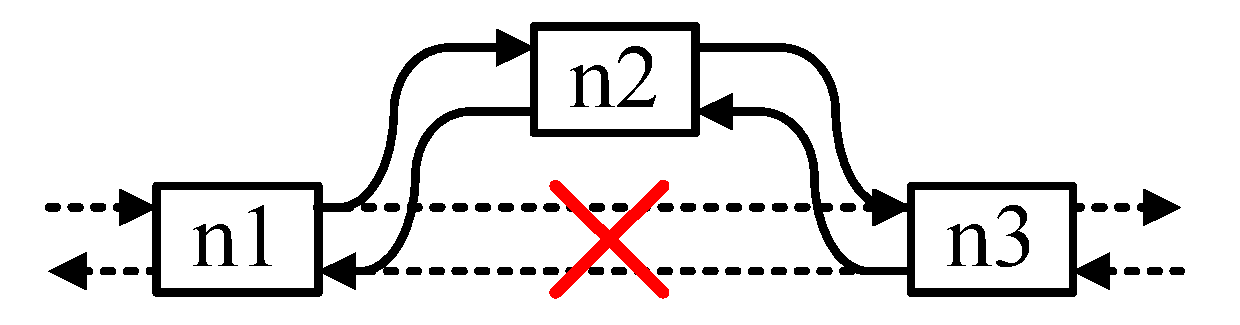
\includegraphics[width=\columnwidth]{images/list_insert.pdf}
			\label{fig:compilation_list_insert}	
		}
		\vspace{1cm}
		\subfloat[remove(n2)]{
			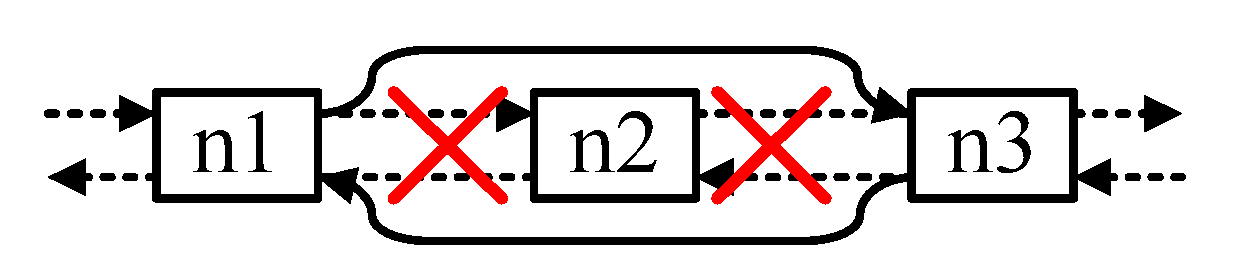
\includegraphics[width=\columnwidth]{images/list_remove.pdf}
			\label{fig:compilation_list_remove}	
		}
	\end{minipage}

	\caption{Definition of a linked list node and its operations.}
	\label{fig:compilation_linkedlist}
\end{figure}

\begin{table}
	\centering
	
	\renewcommand{\arraystretch}{1.25}
	\begin{tabular}{| c | l |}
		\hline
		\textbf{Execution Point}		& \multicolumn{1}{c|}{\textbf{Linked Lists}}																		\\
		\hline
		When the program starts			& \raisebox{0.15cm}{\textbf{Core 1:}} 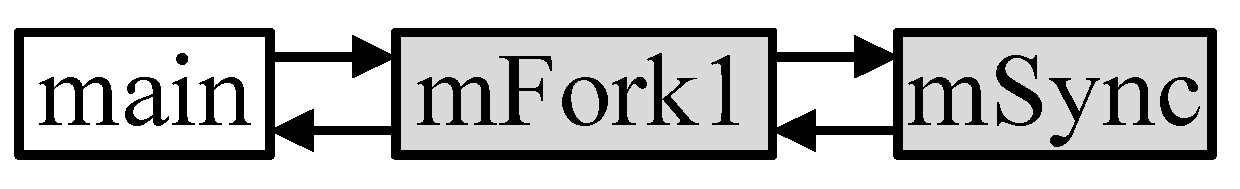
\includegraphics[height=0.55cm]{images/list_m1.pdf}	\\
										& \raisebox{0.15cm}{\textbf{Core 2:}} 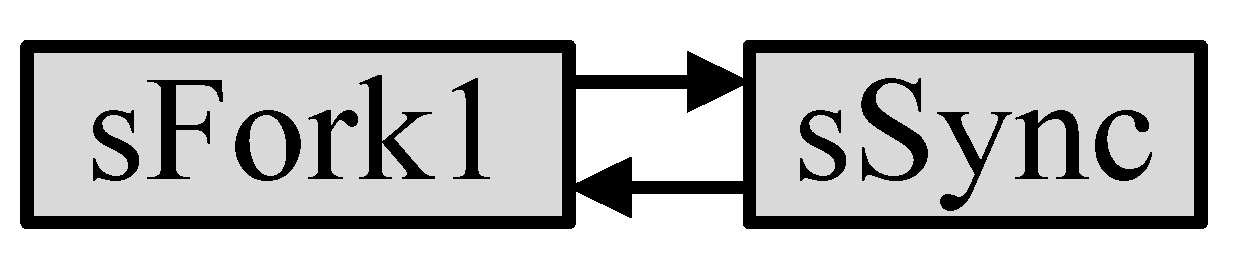
\includegraphics[height=0.55cm]{images/list_s1.pdf}	\\ \hline
		When main \par forks (id = 1)	& \raisebox{0.15cm}{\textbf{Core 1:}} 
\includegraphics[height=0.55cm]{images/list_m2.pdf}	\\
										& \raisebox{0.15cm}{\textbf{Core 2:}} 
\includegraphics[height=0.55cm]{images/list_s2.pdf}	\\ \hline
		When tA \par forks (id = 2)		& \raisebox{0.15cm}{\textbf{Core 1:}} 
\includegraphics[height=0.55cm]{images/list_m3.pdf}	\\
										& \raisebox{0.15cm}{\textbf{Core 2:}} 
\includegraphics[height=0.55cm]{images/list_s3.pdf}	\\
		\hline
	\end{tabular}
	\caption{Core 1 and 2's initial lists and subsequent lists when threads fork.}
	\label{tab:compilation_lists}
\end{table}

Fortunately, the scheduling of a core's threads and routines
can be kept in the correct order using (doubly)
linked lists. Each node (defined in Figure~\ref{fig:compilation_linkednode}) 
in the list represents a thread or
routine and stores its continuation point (\verb$pc$) and
the links to its neighboring nodes (\verb$prev$ and
\verb$next$). A node's \verb$pc$ is initially set to the
start of the thread or routine's body (e.g., lines~\ref{code:compilation_example3_scheduling3}-\ref{code:compilation_example3_scheduling4}). 
Lines~\ref{code:compilation_example3_direct1}-\ref{code:compilation_example3_direct2} creates core 1 and 2's initial lists,
visualized by the second row of Table~\ref{tab:compilation_lists}. Core 1's list
starts with the \verb$main$ thread, followed by the
\verb$mFork1$ and \verb$mSync$ routines, and Core 2's list
starts with the \verb$sFork1$ and then \verb$sSync$
routines. The \verb$mSync$ and \verb$sSync$ routines are
used to synchronize both cores to complete one tick of the
program (see Section~\ref{sec:compilation_sync}). Each core
starts its scheduling by jumping to the
\verb$pc$ of its first node. A thread or routine
performs a context-switch by jumping to the \verb$pc$ of the 
next node. A core will only execute the threads
and routines in its linked list. Thus, inserting or removing
a thread or routine from the list controls whether it
is included or excluded, respectively, from execution. 
Figures~\ref{fig:compilation_list_insert} and 
\ref{fig:compilation_list_remove} illustrate the 
insertion and removal operations defined in 
Figure~\ref{fig:compilation_linkednode}. The
remainder of this section describes how the linked lists are
manipulated to implement the ForeC semantics. 


\subsection{The \texttt{par} Statement}
\label{sec:compilation_par}
Let \verb$id$ be a unique positive integer that identifies a
\verb$par$ statement. The \verb$par$ statement (e.g., 
line~\ref{code:compilation_example3_par1}) is replaced
with C code that: (1) updates the thread's state to be \verb$id$
(line~\ref{code:compilation_example3_state}),
(2) updates the current thread's \verb$pc$ to be
immediately after the \verb$par$ statement 
(line~\ref{code:compilation_example3_join}), and (3)
context-switches to its \verb$mFork$ routine 
(line~\ref{code:compilation_example3_switch}). 
The \verb$mFork$ routine (e.g., line~\ref{code:compilation_example3_mFork1})
removes itself and the parent thread from the linked 
list and inserts the following in its place: the allocated 
child threads and an \verb$mJoin$ routine.
Recall that the slave cores have an \verb$sFork$
routine in their initial linked list. 
The \verb$sFork$ routine (e.g., line~\ref{code:compilation_example3_sFork1})
removes itself from the linked list and inserts the following in its
place: the allocated child threads and an \verb$sJoin$
routine. If the child threads can fork their own threads,
then \verb$mFork$ and \verb$sFork$ routines need to be
inserted into the lists. This ensures that the nested
threads can be forked. Then, a context-switch is made to the
first child thread. E.g., the last two rows of
Table~\ref{tab:compilation_lists} shows core 1 and 2's linked 
lists when \verb$main$ and \verb$tA$ fork 
(lines~\ref{code:compilation_example3_par1} and 
\ref{code:compilation_example3_par2} respectively). 
When no fork occurs, the \verb$mFork$ and \verb$sFork$ 
routines do nothing and context-switch to the next node. 

When a child thread terminates (e.g., line~\ref{code:compilation_example3_term1}), 
it (1) updates its state to \verb$TERM$ (line~\ref{code:compilation_example3_term2}), 
(2) removes itself from the linked list (line~\ref{code:compilation_example3_term3}), 
and (3) context-switches to the next node (line~\ref{code:compilation_example3_term4}).
The resumption of a parent thread when all its child threads
have terminated is handled by the \verb$mJoin$ 
(e.g., line~\ref{code:compilation_example3_mJoin1}) and
\verb$sJoin$ (e.g., line~\ref{code:compilation_example3_sJoin1}) 
routines. When all child threads have terminated, the
\verb$sJoin$ routine removes itself from the linked list and
context-switches to the next node. The \verb$mJoin$ routine:
(1) updates the parent thread's state to \verb$OTHER$, (2) 
inserts the parent thread back into the linked list, and (3)
removes itself from the list. A context-switch is made to the parent
thread, which resumes its execution from after the
\verb$par$ statement. If some child threads have not
terminated, then the \verb$sJoin$ and \verb$mJoin$ routines
do nothing and context-switch to the next node.


\subsection{The \texttt{pause} Statement}
The \verb$pause$ statement (e.g., line~\ref{code:compilation_example3_pause1}) 
is replaced with C code that: (1) updates the current thread's \verb$pc$ 
to be immediately after the \verb$pause$ statement (line~\ref{code:compilation_example3_pause2}), 
and (2) context-switches to the next node (line~\ref{code:compilation_example3_pause3}). 
In the next tick, execution will resume from after the \verb$pause$
statement.


\subsection{Shared Variables}
Shared variables are hoisted up to the program's global 
scope to allow all cores to access them. The copies of 
shared variables are implemented as unique global variables 
(e.g., line~\ref{code:compilation_example3_copies}). 
This allows copies from different cores
to be combined together. In each thread, all shared variable 
accesses are replaced by accesses to their copies
(e.g., lines~\ref{code:compilation_example3_x_main} and 
\ref{code:compilation_example3_x_tB}). 
At the start of each local tick (i.e., start of each 
thread body, and after each \verb$pause$ 
and \verb$par$ statement), the shared
variables (e.g., \verb$x$ on line~\ref{code:compilation_example3_user1}) 
are copied (lines~\ref{code:compilation_example3_copy1}, 
\ref{code:compilation_example3_copy2} and 
\ref{code:compilation_example3_copy3} of \verb$main$).
Shared variables are resynchronized using the
hierarchical methodology shown in
Figure~\ref{fig:forec_combine}. This is achieved by using
the \verb$mJoin$ routines to combine their child threads'
copies that satisfy the combine policy (e.g., 
lines~\ref{code:compilation_example3_combine1} and 
\ref{code:compilation_example3_combine2}). Note that the
\verb$mJoin$ routines at the bottom of the thread hierarchy
are always executed before those higher up in the hierarchy.
This is because of the \verb$mJoin$ routine's blocking
behavior and its execution priority in the
linked lists. The \verb$mJoin$ routine at the top of
the thread hierarchy always computes the shared variable's
final value.


\subsection{The \texttt{abort} Statement}
Using the preemption condition, conditional jumps are
inserted after each \verb$pause$ statement (e.g., 
line~\ref{code:compilation_example3_abort2}) in the 
\verb$abort$ body 
(lines~\ref{code:compilation_example3_abort1}-\ref{code:compilation_example3_abort3}). 
If the preemption condition evaluates to true, then 
execution jumps to the statement immediately after the
\verb$abort$. If a \verb$par$ statement is inside
an \verb$abort$ body, then the preemption condition must be
evaluated before the threads can execute. Thus, when a fork
occurs, an \verb$Abort$ routine (e.g., line~\ref{code:compilation_example3_mAbort1}) 
is inserted before the child threads in the linked lists 
(e.g., line~\ref{code:compilation_example3_mAbort1_insert}). The \verb$Abort$
routine evaluates the preemption condition and will
terminate the child threads if it evaluates to true. The
master core's \verb$mAbort$ routine 
(e.g., line~\ref{code:compilation_example3_mAbort1})
also updates the parent thread's \verb$pc$ to be immediately after
the \verb$abort$ statement. Note that it is safe to evaluate the 
preemption conditions in parallel because they are side-effect 
free.


\subsection{Tick Synchronization}
\label{sec:compilation_sync} 
To preserve the notion of a tick, each linked list always
ends with a \verb$sync$ routine (e.g., lines~\ref{code:compilation_example3_mSync}
and \ref{code:compilation_example3_sSync}) that implements barrier
synchronization. Once all cores are 
synchronized, one routine (line~\ref{code:compilation_example3_mSync})
performs the following housekeeping tasks: finalizing the
values of the shared variables, emitting outputs, and sampling
inputs. Then, the next tick is signaled and the cores
execute the threads and routines in their linked list again,
starting from the first node.


%\subsection{Optimizations}
%Inlined nesting of \verb$par$ statements (each nested 
%\verb$par$ statement is not in sequence with any other 
%statement): Fork and join all the nested threads together.
%
%Shared variable that does not need a combine function: Assign
%the writer's copy directly to the shared variable.
%
%Shared variable that is only read by a thread: Apart from the
%thread's first local tick (where the parent's copy is read), 
%the shared variable can be read in subsequent local ticks.
